\documentclass[DM,authoryear,toc]{lsstdoc}
% lsstdoc documentation: https://lsst-texmf.lsst.io/lsstdoc.html
\input{meta}

% Package imports go here.

% Local commands go here.

%If you want glossaries
%\input{aglossary.tex}
%\makeglossaries

\title{Periodicity Analysis in Alert Production}

% Optional subtitle
% \setDocSubtitle{A subtitle}

\author{%
Anastasios Tzanidakis, Eric Bellm
}

\setDocRef{DMTN-221}
\setDocUpstreamLocation{\url{https://github.com/lsst-dm/dmtn-221}}

\date{\vcsDate}

% Optional: name of the document's curator
% \setDocCurator{The Curator of this Document}

% WIP
\setDocAbstract{%
The baselined timeseries features to be computed in Alert Production include a Lomb-Scargle periodogram. We assess the computational and scientific performance of several configurations on simulated alert data.
}


% Change history defined here.
% Order: oldest first.
% Fields: VERSION, DATE, DESCRIPTION, OWNER NAME.
% See LPM-51 for version number policy.
\setDocChangeRecord{%
  \addtohist{1}{YYYY-MM-DD}{Unreleased.}{Anastasios Tzanidakis, Eric Bellm}
}


\begin{document}

% Create the title page.
\maketitle
% Frequently for a technote we do not want a title page  uncomment this to remove the title page and changelog.
% use \mkshorttitle to remove the extra pages

% ADD CONTENT HERE
% You can also use the \input command to include several content files.

\section{Note}
\textcolor{red}{Please note that this DM-technote is currently work in progress, and publicly available. The final findings will be pushed to the DMTN-221 repository in late November of 2022 by Anastasios Tzanidakis.}


\section{Motivation}
The characterization of periodicity from time-series is a fundamental constraint to numerous astrophysical applications. Phenomenologically, estimating the periodicity and its significance can shed light on stellar pulsation theory \citep{Antonello:Antonello81}, distance estimation and mapping of the Galaxy through the period-luminosity relationship \citep{Skowron:Skowron2019}, constraint fundamental parameters of stellar binaries \citep{Farinella:Farinella1979} and stellar rotation \citep{Walkowicz:Walkowicz13}. In the recent decade, the use of periodicity has also been extensively used as a feature to classify variable phenomena \citep{Richards:R13} across the Hertzsprung-Russell diagram. 

Previous work from \cite{2012AJ....144....9O} demonstrate the concept of injection-recovery test for synthetically generated RR Lyrae templates from SDSS using the op$\_$sim version 1.29 cadence strategy. However, no study to date has demonstrated the recovery period distribution of more complex periodic phenomena such as eclipsing binaries in real-time. In this study, we perform an end-to-end injection-recovery analysis for periodic multi-band time series to asses the statistical significance of period finding in the context of the LSST AP as suggested in \citeds{DMTN-118}.

\section{Synthetic Light Curves}
In this study we use the training set Extended LSST Astronomical Time-series Classification Challenge (ELAsTiCC) light curves with a 12 month history that will best mimic the calculations performed for AP. In short, ELAsTiCC is a real-time pipeline for generating mock photometric alerts at the expected LSST rate. The photometric alerts will be distributed in real-time to brokers to benchmark classification algorithms. The ELAsTiCC dataset uses the v.1.7 cadence strategy from op$\_$sims of the first three years of the survey. A single detection is based on the DIA performance from DC2. Each light curve include photometric noise using Poisson noise that includes the equivalent area, background noise per unit area, sky and CCD read noise. Most importantly, the ELAsTiCC light curves simulate force photometry alerts which we recommend all time series features to be calculated upon. 
	
For this investigation, we use two classes of periodic variable sources: RR Lyrae (RRL) and eclipsing binaries (EB). Both RRL's and EB's represent the extrema of simple and complex periodic sources that will throughly test the underlying ability of the periodogram to find the correct period. While other quasi-periodic sources, such as AGN, might be of importance, in this study we aim to answer if computing the periodogram on periodic phenomena is possible.  

We note one small drawback using the ELAsTiCC training is the relatively small sample size (N=360) and low signal-to-noise ratio for the eclipsing binaries. In Section \ref{sec:limitations} we discuss the implications of the SNR of the EB light curves.To maximize the use different eclipsing binary stars sampled at different phases, each light curve over a three year photometric history is sampled at some random time and ensures that the maximum baseline is less than 12 months. While a small EB sample size limits the search for a larger distribution in periodicities, it remains nonetheless useful to see the periodicity recovery rates at different sampling phases. In Figure \ref{fig:period_distributions}, we show the underlying injected period distribution or both periodic classes. Finally, in Figure \ref{fig:light_curve_demo} we show the typical multi-band AP light curve sampled from ELAsTiCC with uncertainties.

\begin{figure*}
  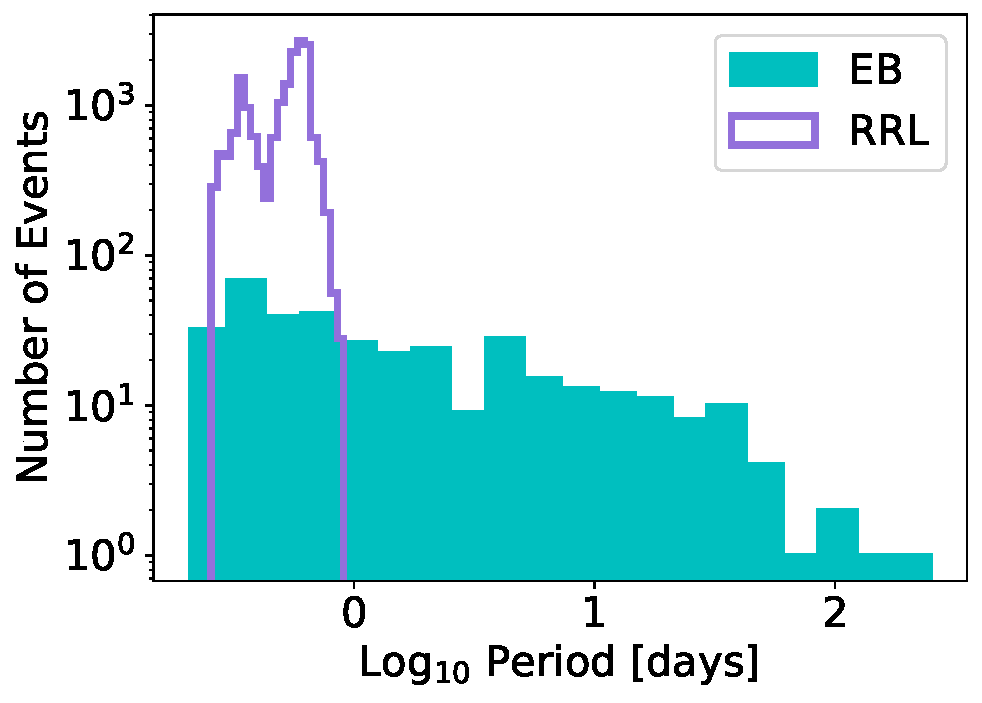
\includegraphics[width=0.5\textwidth]{figures/period_distribution.pdf}
  \centering 
  \caption{True period distribution from the ELAsTiCC training set.}
   \label{fig:period_distributions}
\end{figure*}

\begin{figure*}
  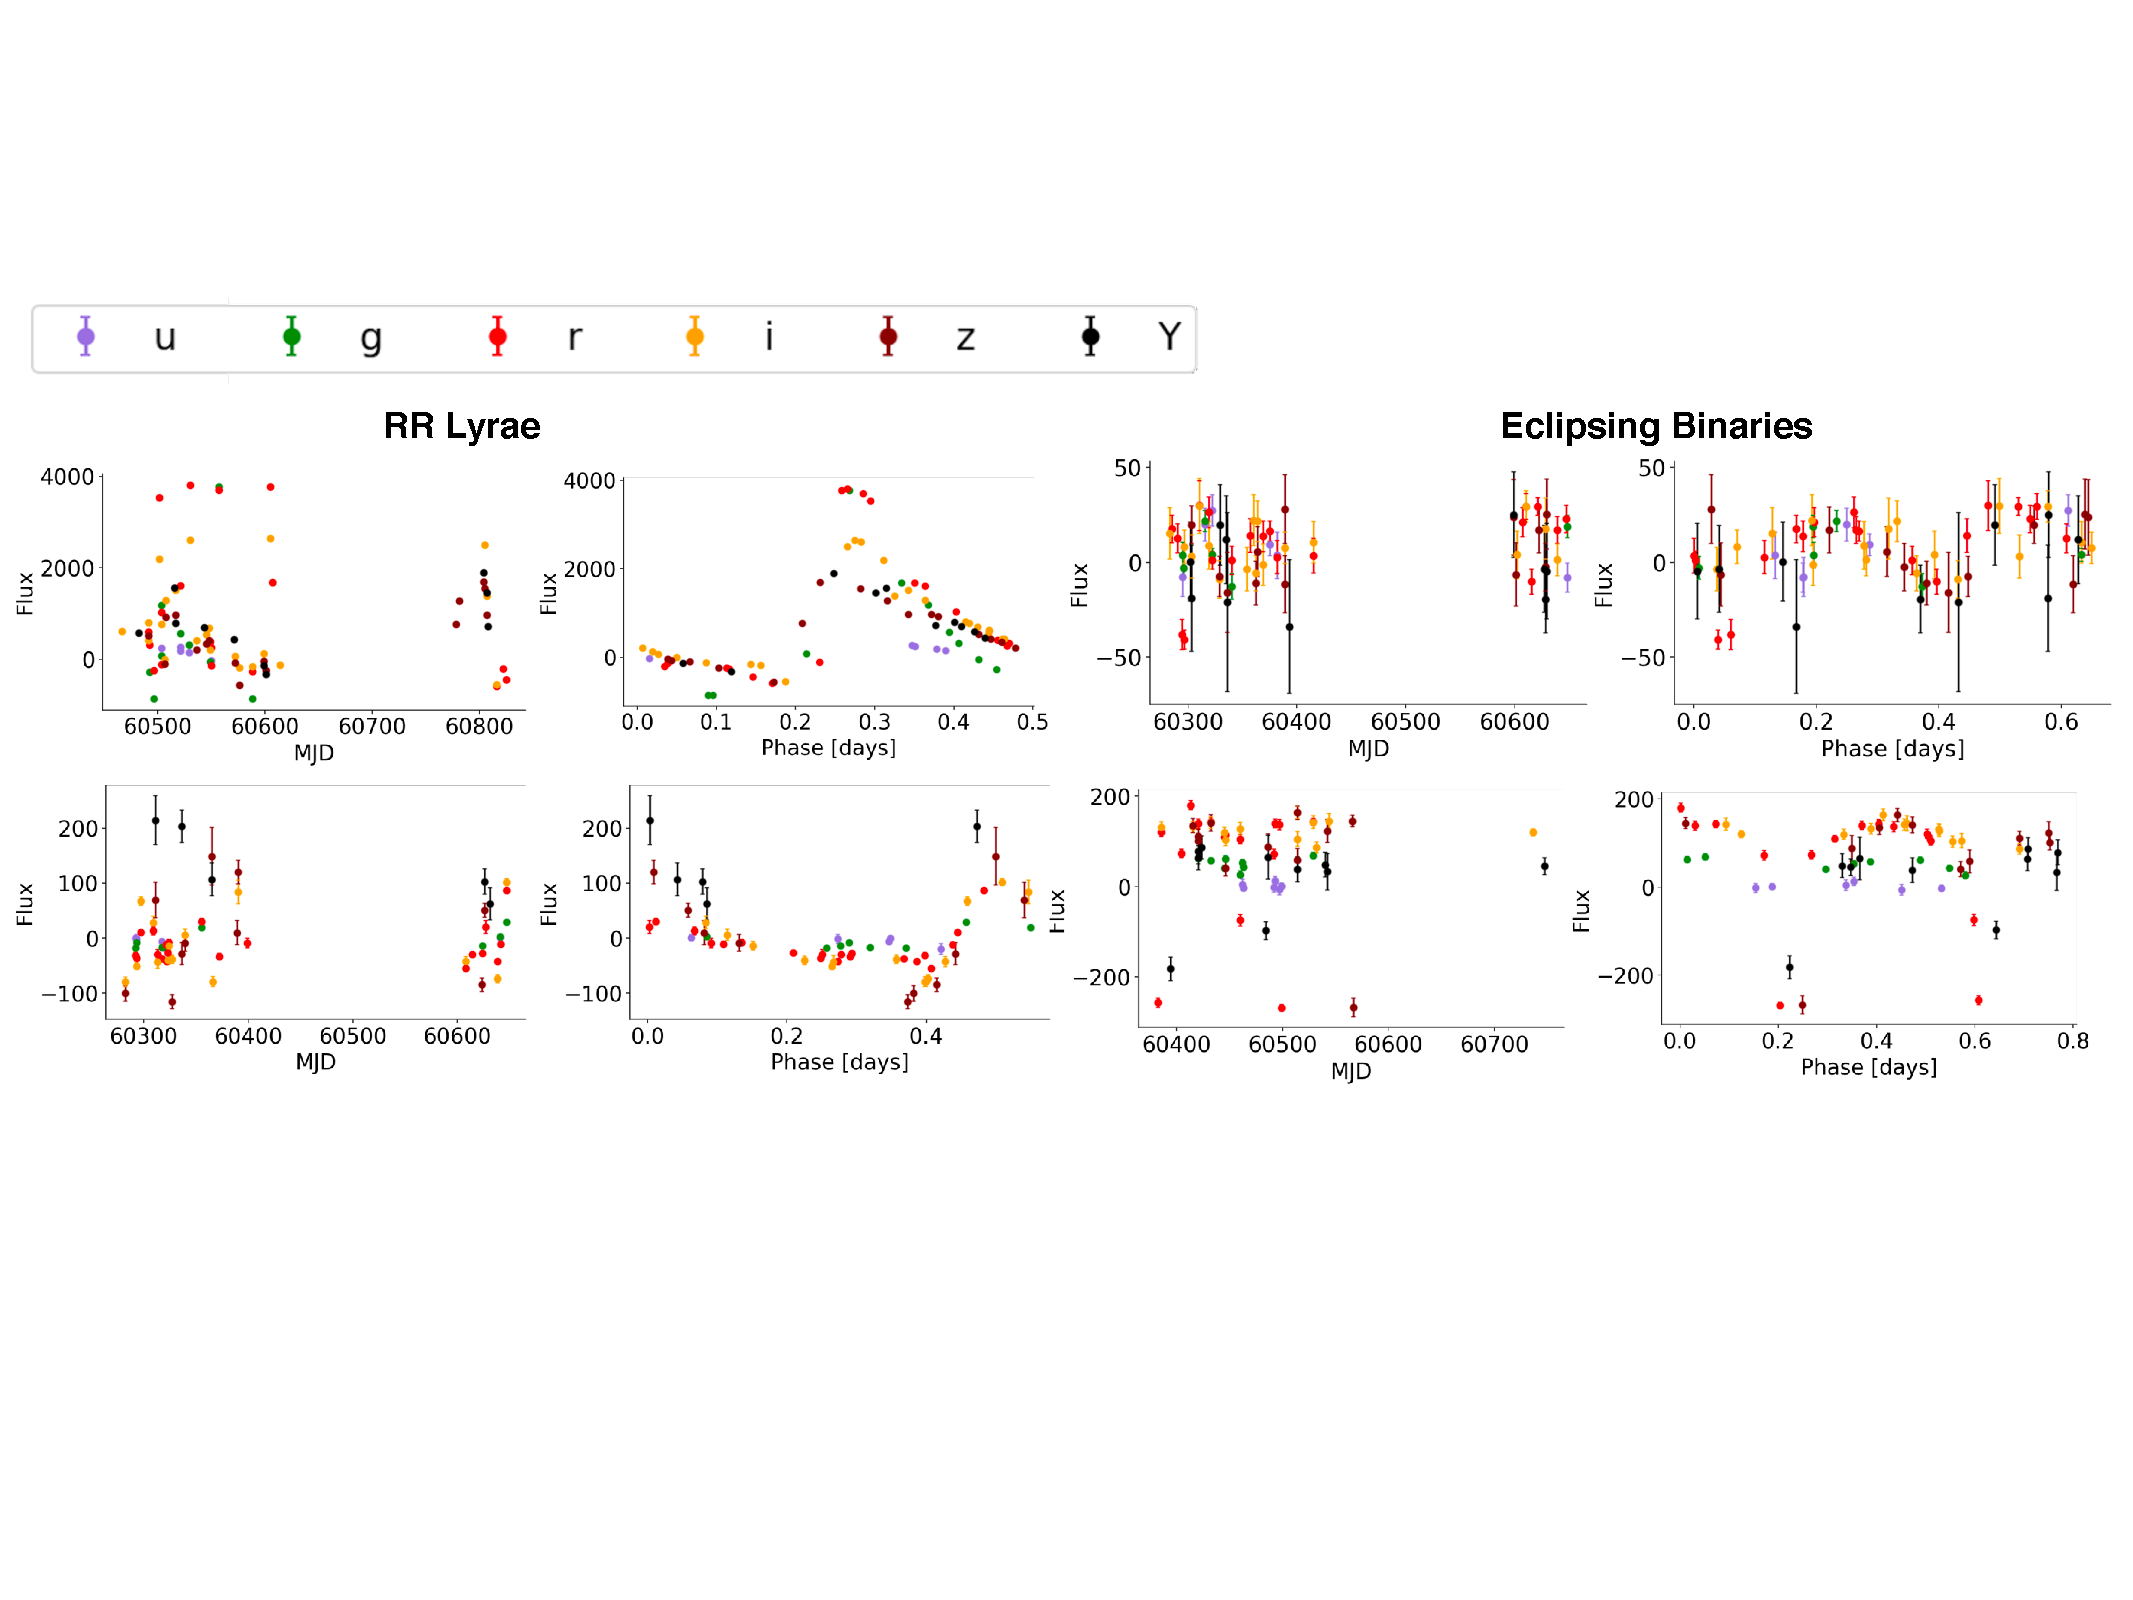
\includegraphics[width=0.9\textwidth]{figures/lightcurve_demo.pdf}
  \centering 
  \caption{The above panels demonstrate the multi-band light curves simulated from ElasTiCC using RR lyrae (left panel) and eclipsing binaries (right panel). The first column of each panel shows the observed light curves, and the second the phase folded light curves at the correct period after 12 months.}
   \label{fig:light_curve_demo}
\end{figure*}

\section{Injection-Recovery Testing}
In this section we discuss the periodicity recovery rate for injected RR Lyrae and eclipsing binaries in both scenarios of single-band and multi-band light curves. All computations of the periodogram henceforth will be the floating-mean Lomb-Scargle periodogram algorithm that is implemented from \textsc{gatspy} \citet{VanderPlas:VP2015}. 

\subsection{Period Grid}
The LSST will be search for periodic phenomena across both short and long timescales. The first challenge when computing periodograms in the context of AP is choosing the right trial period grid with separations that can lead to successful period finding. The periodogram is full of local minima and maxima, thus in practice the global maximum, which corresponds usually to the period with the highest power, is searched through a brute force period grid. High resolution period grids can also be very computationally expensive that is not feasible in the 60 second data latency of AP. 

Inevitably, large searches in period space without an a priori will require an heuristic approach to generating an appropriate period grid that will account for the light curve characteristics. For this study, we use a heuristic frequency grid generator adapted in \textsc{gatspy} that uses the light curve parameters to estimate the appropriate frequency grid length and separation. Unfortunately, for sparsely sampled light curves there does not exist a straightforward approach to finding the optimum frequency grid. It is inevitable that some light curves will either require coarser or finer frequency grids. 
Generally, the frequency separation that we will be using for thus study can be approximated using the duration of the light curve, including some sampling constant ($\mathcal{O}$) and the total number of computed periods as a function of the Nyquist factor ($F_{nyquist}$), and number of detections (N$_{det}$): 

\begin{equation}
\delta f = \frac{1}{(t_{max} - t_{min}) \times \mathcal{O}}
\end{equation}

\begin{equation}
N_{P} = int \bigg{(} \frac{1}{2} \mathcal{O} F_{nyquist} N_{det} \bigg{)}
\end{equation}

Building some intuition, the Nyquist factor pushes the minimum starting frequency to smaller periods while the oversampling factor will increase the maximum frequency grid and overall increase the resolution of the grid. In later sections we evaluate for each frequency grid the period accuracy computed on the ELAsTiCC light curves. 

\subsection{Single Band Lomb-Scargle Periodogram}

We first consider the case of the canonical single-band detections from AP. In this section we aim to answer  if the 12 month AP history in a single-band light curve is enough to recover periods. The reader should refer to \citet{VanderPlas:VP2015} for a throughout review of the Lomb-Scargle periodogram.   

We consider the canonical floating-mean Lomb-Scargle to estimate the periodogram of $10^4$ alert light curves in the \textit{r}-band for three Fourier component modes. For the average LSST field, our results are independent of the selected photometric filter due the uniformity of sky coverage from all filters. In Figure \ref{fig:single_band_lsp} we show the results of this analysis for RRL's (rop row) and EB's (bottom row). For each light curve model, we randomly sample a light curve and compute the Lomb-Scargle periodogram using a heuristic period grid with an oversampling factor of 2 and Nyquist frequency of 30 ($\sim$0.03 days) to account for the fast periodic phenomena. We extrapolated the highest power period from the periodogram and compare it to the true period. In Figure \ref{fig:single_band_lsp} we also include the number of \textit{r}-band detections for each light curve. We note that we did not find any reliable periods beyond 5 days for the eclipsing binaries. This is likely due to the fact of the small sample size beyond 5 days. Since we are re-sampling the same underlying models it is possible that the light curve re-sampling is not aduete enough to identify correct large periods. As expected, we did not find any preference of an optical single-band photometric filter that outperformed the others. While the RR Lyrae exhibit at larger Fourier modeling modes more aliasing, overall the recovery fraction of correctly identified periods is larger compared to the EBs. For both light curve models, we consistently found in each model configuration that the average correctly identified period coincides with a larger number of detections. Overall we find consistent results for the RR Lyrae done by a similar analysis by \citet{VanderPlas:VP2015}. The true challenge of this approach comes from the more complex light curves such as the EBs with more phase variation. 

\begin{figure*}
  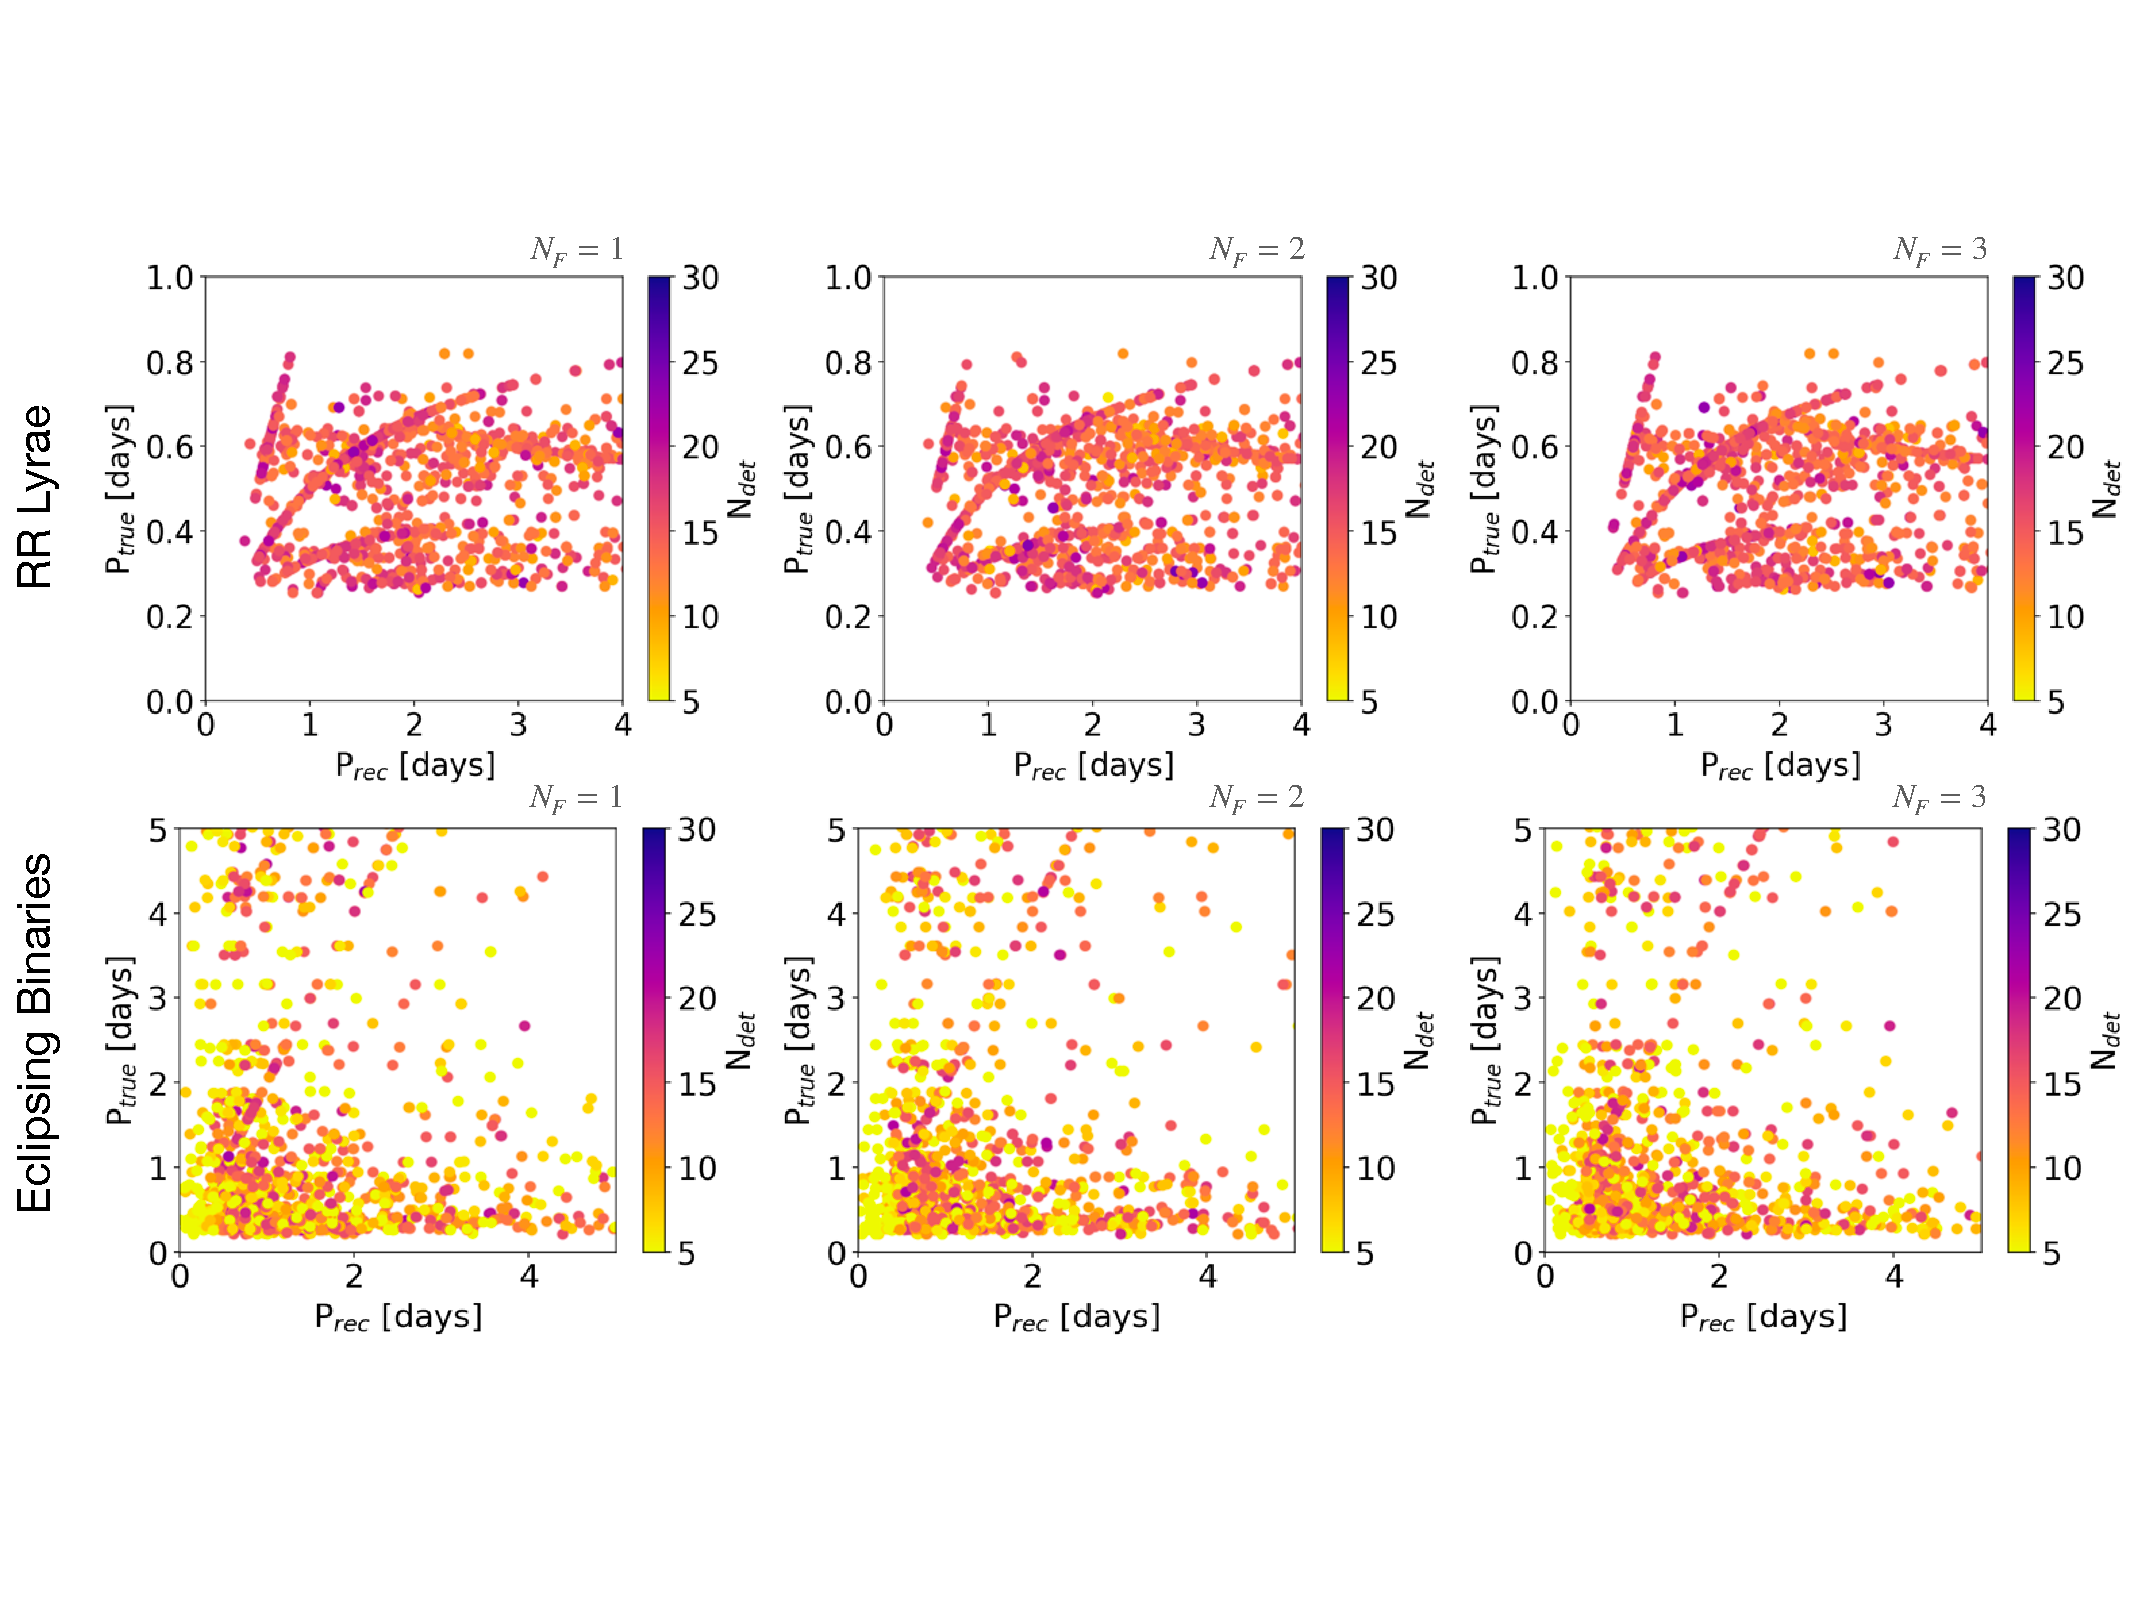
\includegraphics[width=0.7\textwidth]{figures/singleband_lsp.pdf}
  \centering 
  \caption{We show the injected (true period) versus recovered highest peak in the periodogram for a sample of 1000 $r$-band detections from RR lyrae and eclipsing binaries. Each column shows the period recovery for N=1 to N=3 Fourier components when computing the Lomb-Scargle periodogram.}
  \label{fig:single_band_lsp}
\end{figure*}

% Conclusions regarding the single-band Lomb Scargle
On average, there will be 30 detections in each photometric band per 12 month light curve history. Given the sampling rate of LSST per pointing, this entails that the majority of single-band AP light curves would be too undersampled in order to compute a high confidence periodicity. Even with a low completeness, computing the Lomb-Scargle periodogram on single-band time series alerts, this will likely outperform any other known survey due to the large survey volume. The single-band Lomb-implementation are also faster by a factor of 5 due to the lower average number of detections per filter. We conclude that the single-band Lomb-Scargle misses by a higher margin the underlying true period due the small light curve photometric history. We now turn our attention to the multi-band Lomb-Scargle.

\subsection{Multi-Band Lomb-Scargle Periodogram}
Next, we test the multi-band Lomb-Scargle periodogram implementation adapted in \textsc{gatspy} to our ELAsTiCC light curves. Given the rich multi-band alert detections LSST will deliver, we expect that that conventional period finding algorithms to do better due to an increase of number of total detections. In short, the multi-band Lomb-Scargle periodogram we will be considering for this study can be written out with two components that use implemented in \textsc{gatspy} : 

\begin{equation}
\qquad y = \theta_0+\sum_{n=1}^{M_{base}}\left[\theta_{2 n-1} \sin (n \omega t)+\theta_{2 n} \cos (n \omega t)\right] \\
\theta_0^{(k)}+\sum_{n=1}^{M _{band}}\left[\theta_{2 n-1}^{(k)} \sin (n \omega t)+\theta_{2 n}^{(k)} \cos (n \omega t)\right]
\end{equation}

First is the base Fourier component that describes the overall shared variability, and second is the per band component that is modeled by the residuals of the base component with each photometric filter. In practice, a larger configuration of base and band components can lead to the estimation of more complex light curves. \textsc{gatspy} automatically determines through the use of least-squares minimization the scalar parameters from the above equation. For a more detailed mathematical review of the multi-band Lomb-Scargle we suggest the review of \citet{VanderPlas:VP2015}. 

% Discuss the findings of the multi-band LSP (re-do): WIP
% TODO run simulation


% Need to update figure
\begin{figure*}
  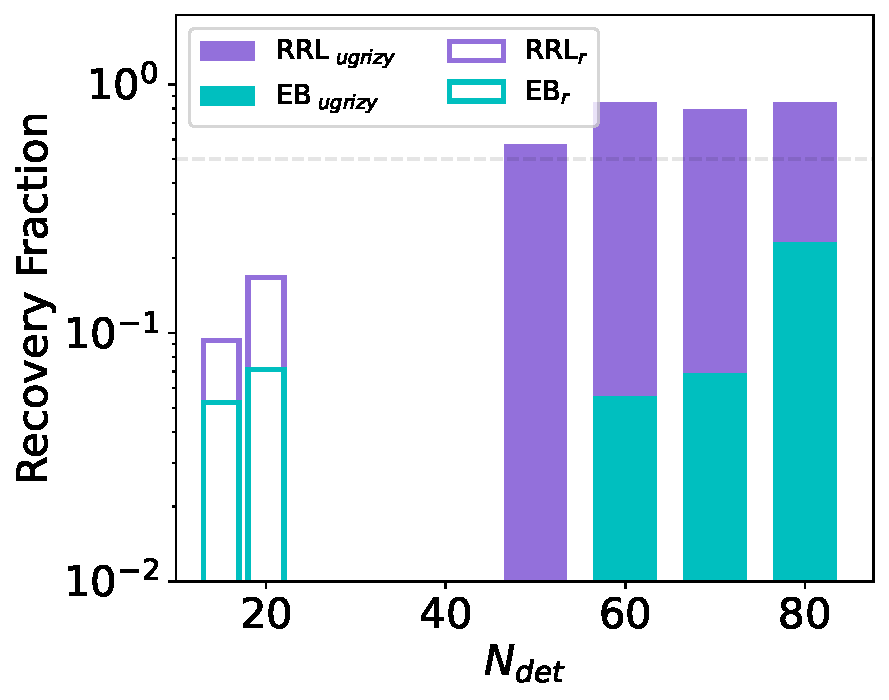
\includegraphics[width=0.6\textwidth]{figures/multi_vs_single_rec_frac.pdf}
  \centering 
  \caption{Multi-band injection-recovery test for 5000 RRL (top row) and EB (bottom row). Each column title includes the number of Fourier base and band terms used to compute the Lomb-Scargle periodogram. Additionally we color code each recovered period by the number of detections. The overlaid curved lines represent the n=1 aliasing, while the straight lines represent the n=1,2 harmonics.}
\end{figure*}

\subsection{Peak Significance Metric}
One imminent challenge beside choosing the right period grid, and model complexity is the reported period significance. It is inevitable that the AP periodic pipeline will likely report spurious periods, and both harmonics and aliases of the underlying period of the source. The effects of aliasing and harmonics are typically identified by visual inspection of the phase folded light curves. In this section we explore empirical metrics to evaluate peak significance within the AP time frame. One common diagnostic used in the literature is the False Alarm Probability (FAP) a given peak in the power spectrum. The FAP measures the probability uncertainty associated with the selected peak under the null hypothesis. Generally, the reported FAP for a specific period peak can be used to inform the user of its a trustworthy detection. A constraint on the number of detections and FAP is adequate to achieve a complete catalogue of periodic phenomena. 

% Bootstraping as a mechanism 
Given the absence of a true analytic solution to the Lomb-Scargle FAP, most methods rely on computational approaches such as bootstrapping. Bootstrapping by virtue is computationally expensive. For example, a 1$\%$ FAP rate would require 1000 bootstraps per light curve. By simply scaling the expected number of periodic sources to be found in each LSST pointing, we find that that the number of computed periodogram to likely exceed the computing resources of AP. Given the fast AP latency and number of periodic sources, a significant real-time bootstraping is likely not feasible for AP. A more popular approach is to use parametric FAP estimators that asymptotically converge to similar distributions of bootstraping FAP approaches. A sophisticated approach suggested by \citet{Baluev:Baluev2008} which uses extreme value statistics to compute an upper bound of the false alarm probability for the alias-free case:

\begin{equation}
P_{FAP} \approx \frac{\Gamma((N-1) / 2)}{\Gamma((N-2) / 2)} \sqrt{4 \pi \operatorname{var}\left(t_i\right)} f_{\mathrm{u}}\left(1-z_{\mathrm{obs}}\right)^{\frac{N-4}{2}} \sqrt{z_{\mathrm{obs}}}
\end{equation}

The Baluev approximation has already been applied in other studies such as \citet{Suveges:Suveges15} and is suggested as a computationally inexpensive and reliable form to approximate the FAP. The more complex issue arrises from the complex mathematics that involve the derivation of the Baluev approximation for the multi-band Lomb-Scargle form. The derivation of such form is beyond the scope of this paper, and we suggest future studies to explore if such solution exists. For practical purposes, in our case we assume that the \citet{Baluev:Baluev2008}  form will hold true for the multi-band case, however we caution that the overall FAP estimates to possibly be underestimated or overestimated. 


To test whether the Baulev approximation holds true for the multi-band light curves we attempt to correlate a conventional bootstraping significance approach with the Baluev form. We begin with a 500 light curve sample of RRL and EB assuming a (N$_{base}$, N$_{band}$)=(2,1) model configuration. For each light curve, we run the multi-band Lomb-Scargle implementation 1000 times by sampling the light curve without replacement and extrapolate the maximum power for each iteration. Finally, we compute the ratio between the recovered power of the original Lomb-Scargle periodogram and the median bootstrapped power, which can be interpreted as a significance estimator. In Figure \ref{fig:boot}, we show the correlation between the Baluev and bootstrap approach for each variable class and color-coded by the number of \textit{ugrizy} detections. For each variable class, we ran a Pearson-R correlation test and found in both cases a a negative r-slope with p-value significance p$\ll$ 0.005.

\begin{figure*}
  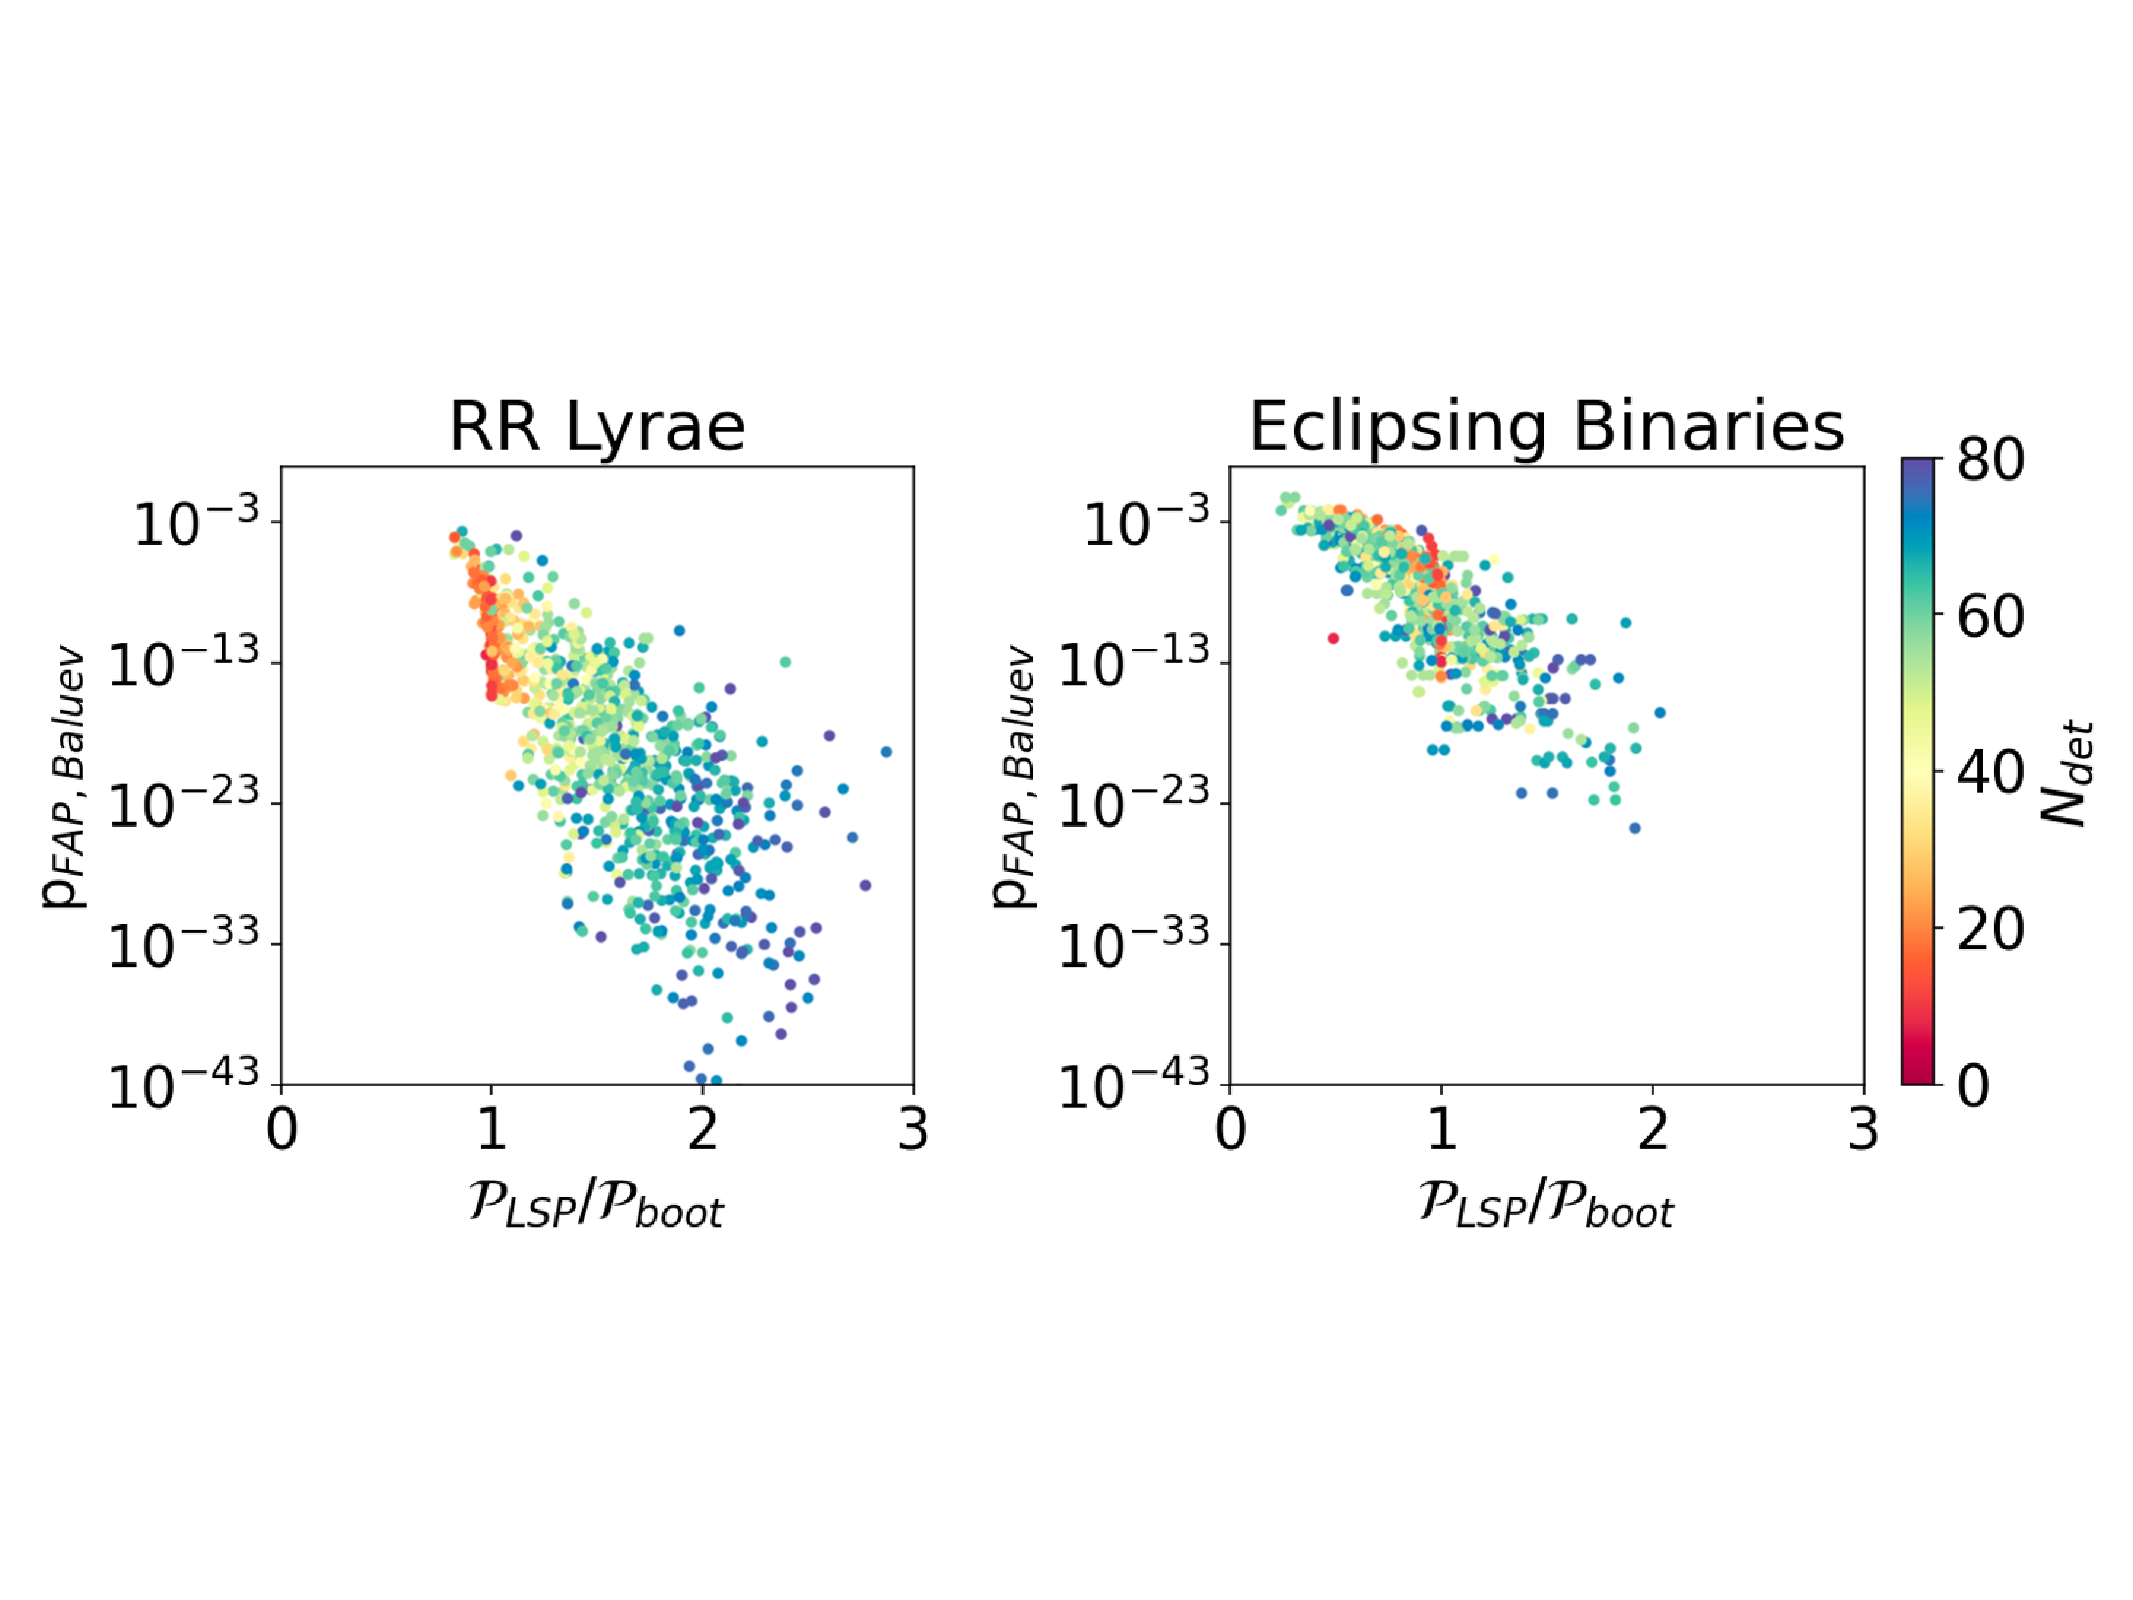
\includegraphics[width=0.8\textwidth]{figures/fap_approximation_mlsp.pdf}
  \centering 
  \caption{Multi-band FAP rate computed via the Baluev approximation compared to a $2\sigma$ bootstrap approach for 5000 RRL and EB alert light curves. For each light curve we also color code the total number of $ugrizy$ detections.}
  \label{fig:boot}
\end{figure*}


% Summary: Timing analysis will include details on bench marking the run time of each frequency grid and model as a function of number of detections and period accuracy.
\subsection{Timing Analysis}

% Introduction
In this section we bench mark the average run time of the Lomb-Scargle periodogram implementation from gatspy. The balancing act of high periodocity accuracy while confining the calculations within the AP timeframe is a challenging act. While coarse period grids  and complex models can achieve more accurate periods, this will not be possible to do with AP. Instead, in this section we will explore the lower limit of run time while tweaking the overall period grid coarseness and model complexity.

The current gatspy, which is a pure Python based implementation of the Lomb-Scargle periodogram, scales as  $\mathcal{O}$[N] algorithm for small N and becomes $\mathcal{O}$[N$^2$] at larger trial periods. The unique rapid calculation of the periodogram emerges from the efficient use of linear algebraic operations. The average run time also depends on the number of detections and model complexity which we will explore in this section. For our run time analysis we will consider both a single-band and multi-band case for the RR Lyrae only since the run time is not a function of the underlying signal. 

% Discussion of single-band 
We first measure the effects of run time on the single-band RRL photometry in the $r$-band filter. In practice, this would work for any given filter given the rolling cadence of LSST. For each light curve, we run the Lomb-Scargle periodogram 10 times per light curve, and compute the median run time. Additionally, we run this for each combination of oversampling factor, Nyquist frequency, and Fourier components. In Figure \ref{fig:run_time_single}, we display the results for the single-band photometry. We also color code the average fractional error per light curve iteration. As mentioned in the single-band Lomb-Scargle method, by design will be poorly sampled especially within the 12 month history. As expected, due to the sparse sampled light curves, the majority of light curves scale linearly with number of detections, and have average run times below one second. 


 
 \begin{figure*}
  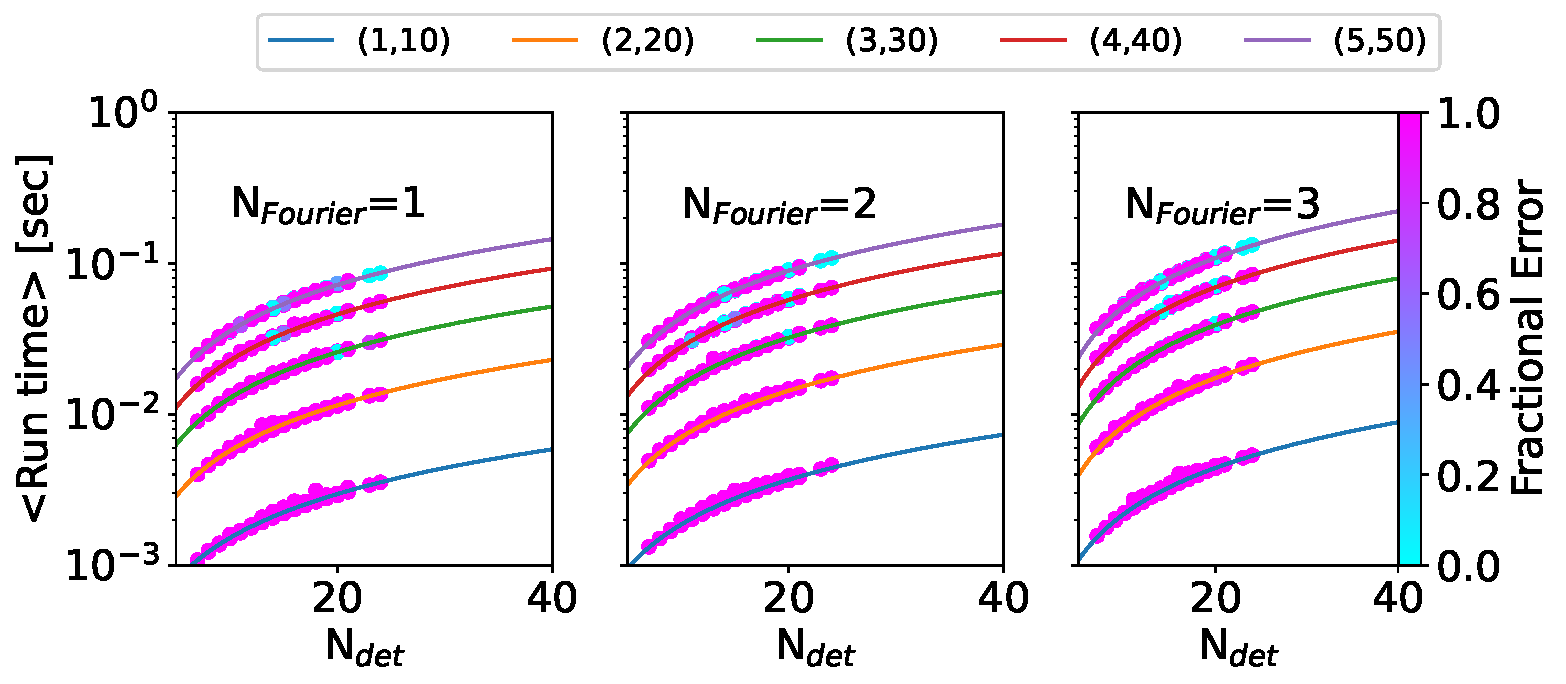
\includegraphics[width=0.8\textwidth]{figures/singleRUN_LSP_RRL.pdf}
  \centering 
  \caption{Average run time per number of $r$ light curve detections. Each column represents the model complexity of each multi-band Lomb Scargle periodogram. Within each panel, we use a heuristically determined period grid by varying the oversampling factor and the the Nyquist frequency.  Finally, for each successive run we color code the fractional error compared from the true period.}
  \label{fig:run_time_single}
\end{figure*}

% Discussion of multi-band

% Conclusions & recommendations  

\begin{figure*}
  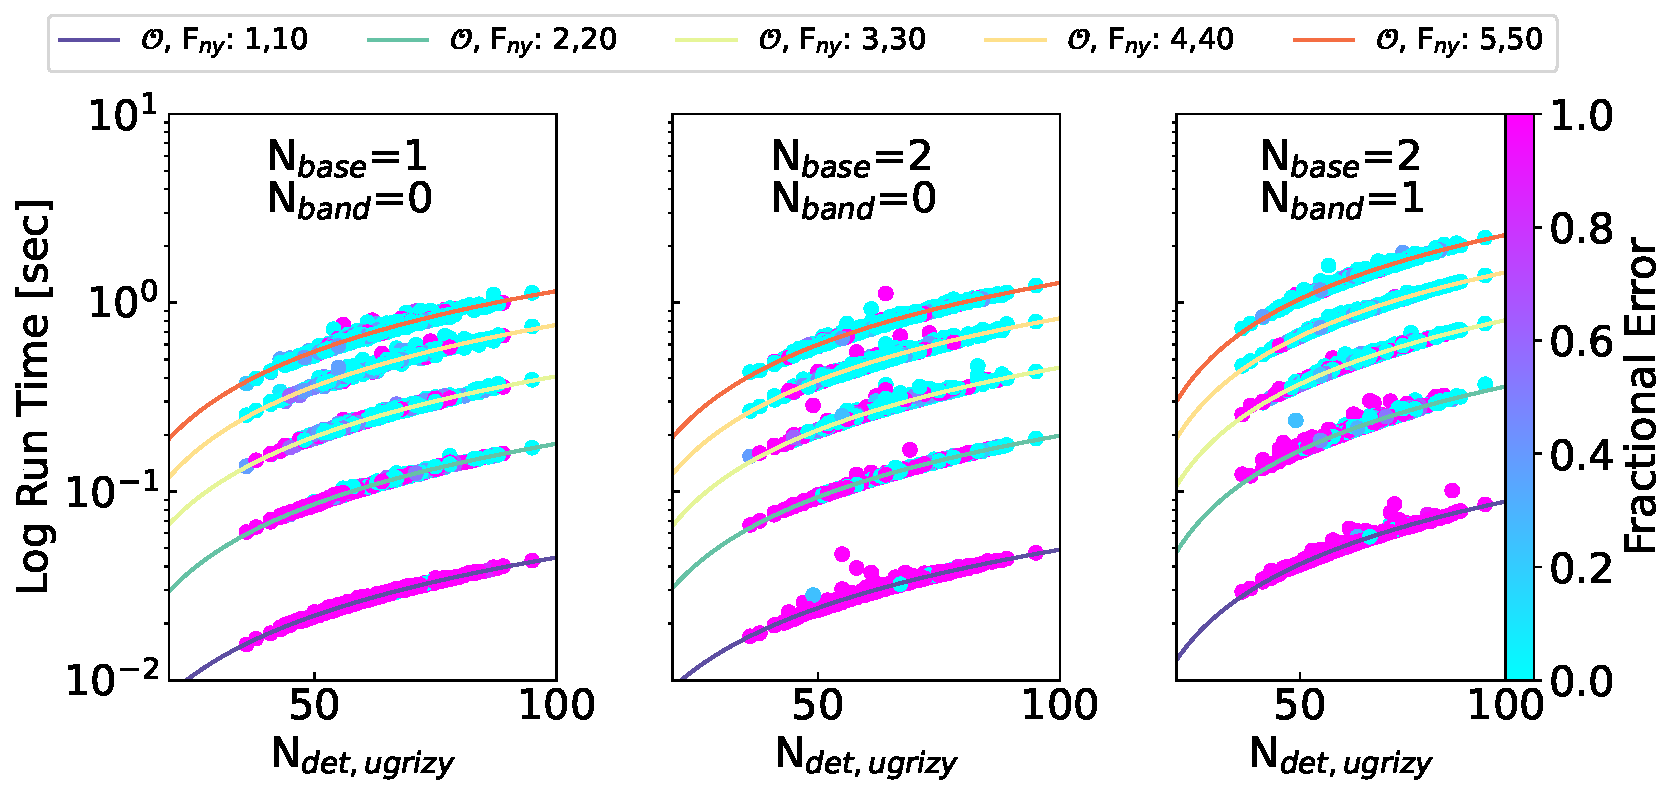
\includegraphics[width=0.8\textwidth]{figures/multi-lsp-runs.pdf}
  \centering 
  \caption{Average run time per number of $ugrizy$ light curve detections. Each column represents the model complexity of each multi-band Lomb Scargle periodogram. Within each panel, we use a heuristically determined period grid by varying the oversampling factor and the the Nyquist frequency.  Finally, for each successive run we color code the fractional error compared from the true period.}
\end{figure*}

\subsection{Current Limitations}\label{sec:limitations}

% Limitations to the Elasticc dataset 
From our analysis, it is evident that the eclipsing binaries overall lack completeness in both cases of single and multi-band. We suspect that the main culpruit of low completeness to be the average low SNR that computed for the ELAsTiCC eclipsing binary sample. For example, in Figure \ref{fig:snr_average}, we show for a sample of 300 ELAsTiCC light curves that the average SNR for the RRL versus EB's to differ by a factor of 50. 

To validate a possible scenario of higher SNR for the eclipsing binaries, using an in-house tool we preliminary... In Figure \ref{fig:multi_lsp_custom} we show the injected versus recovered period for our custom light curves with overall higher SNR. In this case we see that the 

\begin{figure*}
  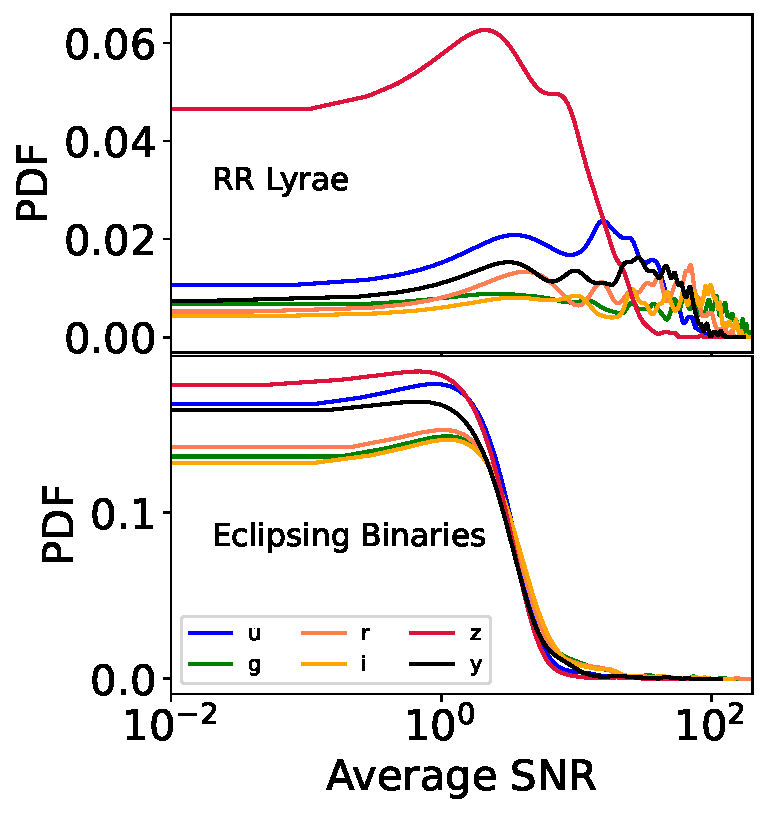
\includegraphics[width=0.7\textwidth]{figures/snr_average.pdf}
  \centering 
  \caption{We compute the median signal-to-noise ratio per light curve in the $ugrizy$ bandpasses.  We smoothen each distribution using a Gaussian Kernel Density estimator. Top panel is the RR Lyrae and bottom is the Eclipsing Binaries. }
  \label{fig:snr_average}
\end{figure*}


\begin{figure*}
  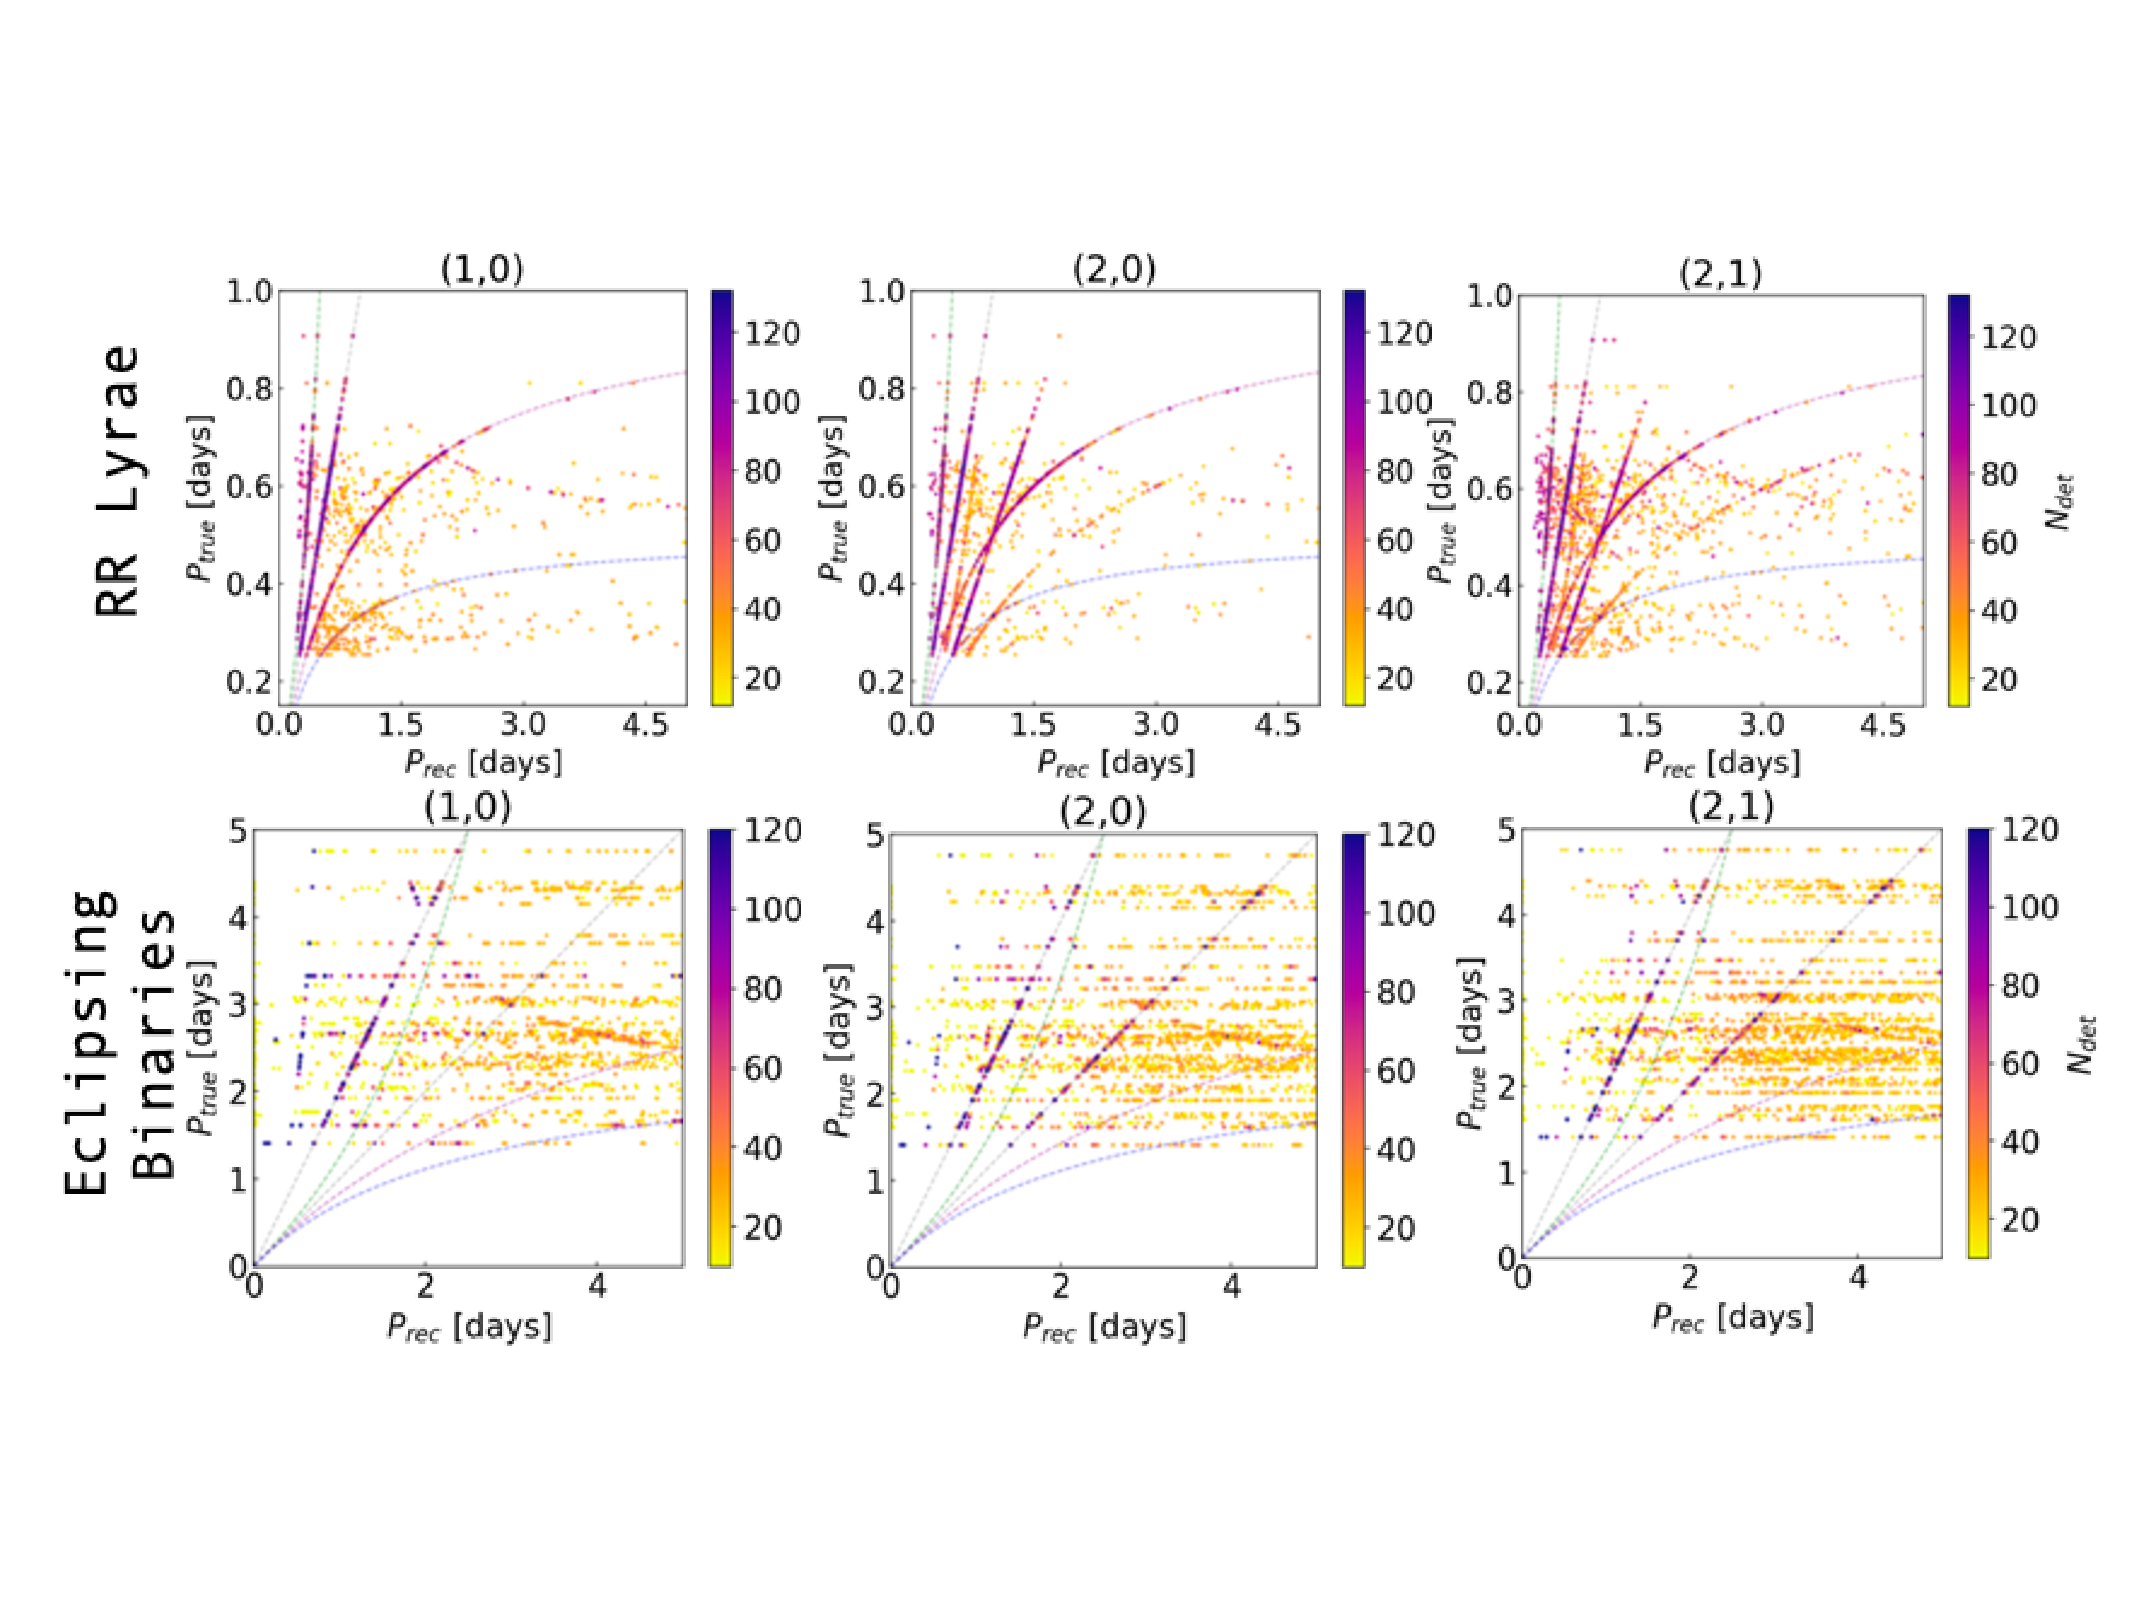
\includegraphics[width=0.9\textwidth]{figures/multi_lsp_rectest.pdf}
  \centering 
  \caption{Multi-band injection-recovery test for 5000 RRL (top row) and EB (bottom row). Each column title includes the number of Fourier base and band terms used to compute the Lomb-Scargle periodogram. Additionally we color code each recovered period by the number of detections. The overlaid curved lines represent the n=1 aliasing, while the straight lines represent the n=1,2 harmonics.}
  \label{fig:multi_lsp_custom}
\end{figure*}



Future investigations prior to the onset of the LSST should investigate a larger suite of eclipsing binary populations at higher luminosities and more throughout  combinations of physical parameters. 

\subsection{Conclusions}

We present a systematic study of periodicity recovery for synthetic LSST AP light curves for RR Lyrae and Eclipsing Binaries.

Overall, we find that 


\appendix
% Include all the relevant bib files.
% https://lsst-texmf.lsst.io/lsstdoc.html#bibliographies
\section{References} \label{sec:bib}
\bibliography{local,lsst,lsst-dm,refs_ads,refs,books}

% Make sure lsst-texmf/bin/generateAcronyms.py is in your path
\section{Acronyms} \label{sec:acronyms}
\addtocounter{table}{-1}
\begin{longtable}{p{0.145\textwidth}p{0.8\textwidth}}\hline
\textbf{Acronym} & \textbf{Description}  \\\hline

AGN & active galactic nuclei \\\hline
CCD & Charge-Coupled Device \\\hline
DC2 & Data Challenge 2 (DESC) \\\hline
DIA & Difference Image Analysis \\\hline
DM & Data Management \\\hline
DMTN & DM Technical Note \\\hline
EB & ExaByte \\\hline
HR & Human Resources \\\hline
LSST & Legacy Survey of Space and Time (formerly Large Synoptic Survey Telescope) \\\hline
SDSS & Sloan Digital Sky Survey \\\hline
\end{longtable}






\end{document}
